%!TEX TS-program = xelatex
\documentclass[10pt,oneside]{article}
\usepackage[fontsize=9pt]{scrextend}

\usepackage[english]{babel}

\usepackage{amsmath,amssymb,amsfonts}
\usepackage[utf8]{inputenc}
\usepackage[T1]{fontenc}
\usepackage{stix2}
\usepackage[scaled]{helvet}
\usepackage[scaled]{inconsolata}

\usepackage{lastpage}

\usepackage{gensymb}

\usepackage{setspace}

\usepackage{ccicons}

\usepackage[hang,flushmargin]{footmisc}

\usepackage{geometry}

\setlength{\parindent}{0pt}
\setlength{\parskip}{6pt plus 2pt minus 1pt}

\usepackage{fancyhdr}
\renewcommand{\headrulewidth}{0pt}\providecommand{\tightlist}{%
  \setlength{\itemsep}{0pt}\setlength{\parskip}{0pt}}

\makeatletter
\newcounter{tableno}
\newenvironment{tablenos:no-prefix-table-caption}{
  \caption@ifcompatibility{}{
    \let\oldthetable\thetable
    \let\oldtheHtable\theHtable
    \renewcommand{\thetable}{tableno:\thetableno}
    \renewcommand{\theHtable}{tableno:\thetableno}
    \stepcounter{tableno}
    \captionsetup{labelformat=empty}
  }
}{
  \caption@ifcompatibility{}{
    \captionsetup{labelformat=default}
    \let\thetable\oldthetable
    \let\theHtable\oldtheHtable
    \addtocounter{table}{-1}
  }
}
\makeatother

\usepackage{array}
\newcommand{\PreserveBackslash}[1]{\let\temp=\\#1\let\\=\temp}
\let\PBS=\PreserveBackslash

\usepackage[breaklinks=true]{hyperref}
\hypersetup{colorlinks,%
citecolor=blue,%
filecolor=blue,%
linkcolor=blue,%
urlcolor=blue}
\usepackage{url}

\usepackage{caption}
\setcounter{secnumdepth}{0}
\usepackage{cleveref}

\usepackage{graphicx}
\makeatletter
\def\maxwidth{\ifdim\Gin@nat@width>\linewidth\linewidth
\else\Gin@nat@width\fi}
\makeatother
\let\Oldincludegraphics\includegraphics
\renewcommand{\includegraphics}[1]{\Oldincludegraphics[width=\maxwidth]{#1}}

\usepackage{longtable}
\usepackage{booktabs}

\usepackage{color}
\usepackage{fancyvrb}
\newcommand{\VerbBar}{|}
\newcommand{\VERB}{\Verb[commandchars=\\\{\}]}
\DefineVerbatimEnvironment{Highlighting}{Verbatim}{commandchars=\\\{\}}
% Add ',fontsize=\small' for more characters per line
\usepackage{framed}
\definecolor{shadecolor}{RGB}{248,248,248}
\newenvironment{Shaded}{\begin{snugshade}}{\end{snugshade}}
\newcommand{\KeywordTok}[1]{\textcolor[rgb]{0.13,0.29,0.53}{\textbf{#1}}}
\newcommand{\DataTypeTok}[1]{\textcolor[rgb]{0.13,0.29,0.53}{#1}}
\newcommand{\DecValTok}[1]{\textcolor[rgb]{0.00,0.00,0.81}{#1}}
\newcommand{\BaseNTok}[1]{\textcolor[rgb]{0.00,0.00,0.81}{#1}}
\newcommand{\FloatTok}[1]{\textcolor[rgb]{0.00,0.00,0.81}{#1}}
\newcommand{\ConstantTok}[1]{\textcolor[rgb]{0.00,0.00,0.00}{#1}}
\newcommand{\CharTok}[1]{\textcolor[rgb]{0.31,0.60,0.02}{#1}}
\newcommand{\SpecialCharTok}[1]{\textcolor[rgb]{0.00,0.00,0.00}{#1}}
\newcommand{\StringTok}[1]{\textcolor[rgb]{0.31,0.60,0.02}{#1}}
\newcommand{\VerbatimStringTok}[1]{\textcolor[rgb]{0.31,0.60,0.02}{#1}}
\newcommand{\SpecialStringTok}[1]{\textcolor[rgb]{0.31,0.60,0.02}{#1}}
\newcommand{\ImportTok}[1]{#1}
\newcommand{\CommentTok}[1]{\textcolor[rgb]{0.56,0.35,0.01}{\textit{#1}}}
\newcommand{\DocumentationTok}[1]{\textcolor[rgb]{0.56,0.35,0.01}{\textbf{\textit{#1}}}}
\newcommand{\AnnotationTok}[1]{\textcolor[rgb]{0.56,0.35,0.01}{\textbf{\textit{#1}}}}
\newcommand{\CommentVarTok}[1]{\textcolor[rgb]{0.56,0.35,0.01}{\textbf{\textit{#1}}}}
\newcommand{\OtherTok}[1]{\textcolor[rgb]{0.56,0.35,0.01}{#1}}
\newcommand{\FunctionTok}[1]{\textcolor[rgb]{0.00,0.00,0.00}{#1}}
\newcommand{\VariableTok}[1]{\textcolor[rgb]{0.00,0.00,0.00}{#1}}
\newcommand{\ControlFlowTok}[1]{\textcolor[rgb]{0.13,0.29,0.53}{\textbf{#1}}}
\newcommand{\OperatorTok}[1]{\textcolor[rgb]{0.81,0.36,0.00}{\textbf{#1}}}
\newcommand{\BuiltInTok}[1]{#1}
\newcommand{\ExtensionTok}[1]{#1}
\newcommand{\PreprocessorTok}[1]{\textcolor[rgb]{0.56,0.35,0.01}{\textit{#1}}}
\newcommand{\AttributeTok}[1]{\textcolor[rgb]{0.77,0.63,0.00}{#1}}
\newcommand{\RegionMarkerTok}[1]{#1}
\newcommand{\InformationTok}[1]{\textcolor[rgb]{0.56,0.35,0.01}{\textbf{\textit{#1}}}}
\newcommand{\WarningTok}[1]{\textcolor[rgb]{0.56,0.35,0.01}{\textbf{\textit{#1}}}}
\newcommand{\AlertTok}[1]{\textcolor[rgb]{0.94,0.16,0.16}{#1}}
\newcommand{\ErrorTok}[1]{\textcolor[rgb]{0.64,0.00,0.00}{\textbf{#1}}}
\newcommand{\NormalTok}[1]{#1}

\newlength{\cslhangindent}
\setlength{\cslhangindent}{1.5em}
\newlength{\csllabelwidth}
\setlength{\csllabelwidth}{3em}
\newenvironment{CSLReferences}[2] % #1 hanging-ident, #2 entry spacing
 {% don't indent paragraphs
  \setlength{\parindent}{0pt}
  % turn on hanging indent if param 1 is 1
  \ifodd #1 \everypar{\setlength{\hangindent}{\cslhangindent}}\ignorespaces\fi
  % set entry spacing
  \ifnum #2 > 0
  \setlength{\parskip}{#2\baselineskip}
  \fi
 }%
 {}
\usepackage{calc} % for \widthof, \maxof
\newcommand{\CSLBlock}[1]{#1\hfill\break}
\newcommand{\CSLLeftMargin}[1]{\parbox[t]{\maxof{\widthof{#1}}{\csllabelwidth}}{#1}}
\newcommand{\CSLRightInline}[1]{\parbox[t]{\linewidth}{#1}}
\newcommand{\CSLIndent}[1]{\hspace{\cslhangindent}#1}\usepackage[table,dvipsnames]{xcolor}

\geometry{includemp,
            letterpaper,
            top=2.4cm,
            bottom=2.4cm,
            left=1.0cm,
            right=1.0cm,
            marginparwidth=5cm,
            marginparsep=1.0cm}

\usepackage[singlelinecheck=off]{caption}

\captionsetup{
  font={small},
  labelfont={bf},
  format=plain,
  labelsep=quad
}

\usepackage{floatrow}

\floatsetup[figure]{margins=hangright,
              facing=no,
              capposition=beside,
              capbesideposition={center,outside},
              floatwidth=\textwidth}

% \floatsetup[table]{margins=hangright,
%              facing=no,
%              capposition=beside,
%              capbesideposition={center,outside},
%              floatwidth=\textwidth}

\pagestyle{plain}

\setcounter{secnumdepth}{5}

\usepackage{titlesec}

\titleformat{\section}[block]
{\normalfont\large\sffamily}
{\thesection}{.5em}{\titlerule\\[.8ex]\bfseries}

\titleformat{\subsection}[runin]
{\normalfont\fontseries{b}\selectfont\filright\sffamily}
{\thesubsection.}{.5em}{}

\titleformat{\subsubsection}[runin]
{\normalfont\itshape\rmfamily\bfseries}{\thesubsubsection}{1em}{}

\fancypagestyle{firstpage}
{
   \fancyhf{}
   \renewcommand{\headrulewidth}{0pt}
   \fancyfoot[R]{\footnotesize\ccby}
   \fancyfoot[L]{\footnotesize\sffamily\today}
}

\fancypagestyle{normal}
{
  \fancyhf{}
  \fancyfoot[R]{\footnotesize\sffamily\thepage\ of \pageref*{LastPage}}
}

\usepackage{tikz}
\begin{document}
\tikz [remember picture, overlay] %
\node [shift={(-0.6in,1.1cm)},scale=0.2,opacity=0.4] at (current page.south east)[anchor=south east]{
\includegraphics{logo}};%
\pagestyle{normal}
\thispagestyle{firstpage}

\newcommand{\colorRule}[3][black]{\textcolor[HTML]{#1}{\rule{#2}{#3}}}

\noindent {\LARGE \textbf{\textsf{Inter-ecosystem specifications of
energy transfer in trophic interactions}}}

\medskip
\begin{flushleft}
{\small
%
\href{https://orcid.org/0000-0002-4104-9463}{Benjamin\,Mercier}%
%
\,\textsuperscript{1,2,‡}
\vskip 1em
\textsuperscript{1}\,Université de
Sherbrooke; \textsuperscript{2}\,Québec Centre for Biodiversity
Sciences\\
\textsuperscript{‡}\,Equal contributions\\
\vskip 1em
\textbf{Correspondance to:}\\
Benjamin Mercier --- \texttt{benjamin.b.mercier@usherbrooke.ca}\\
}
\end{flushleft}

\vskip 2em
\makebox[0pt][l]{\colorRule[CCCCCC]{2.0\textwidth}{0.5pt}}
\vskip 2em
\noindent

\marginpar{\vskip 1em\flushright
{\small{\bfseries Keywords}:\par
trophic interactions\\energy fluxes\\ecosystem\\}
}


This is a very short abstract




\vskip 2em
\makebox[0pt][l]{\colorRule[CCCCCC]{2.0\textwidth}{0.5pt}}
\vskip 2em

\hypertarget{introduction}{%
\section{Introduction}\label{introduction}}

\begin{itemize}
\item
  prey predator relations
\item
  allometry
\end{itemize}

The space clearance rate, as defined by (DeLong 2021), is a parameter
involved in the action of predation. Following its name, the units of
the parameter are of area cleared (km²) per individual per unit of time
(year).

We know that the maximum speed of an organism scales with its bodymass
(Hirt \emph{et al.} 2017). Therefore, we assume that the space clearance
rate of a organism scales with its maximum speed. In this study we found
that the space clearance rate of an organism scales with its bodymass.

\begin{itemize}
\item
  See (Brown \& Gillooly 2003) for rate of interaction depends on the
  rate of metabolism which depends on body size and temperature. He also
  said that rate of interspecific interaction can be predicted by the
  metabolic theory, because rate of consumption and growth are
  determined by individual metabolic rates and have the same
  dependencies on body sizes and temperature.
\item
  Paper de Gibert ou Gilbert?
\item
  Check model Loreau
\item
  Brose 2010 pour v \textasciitilde{} M
\end{itemize}

\hypertarget{method-description}{%
\section{Method description}\label{method-description}}

\hypertarget{the-data}{%
\subsection{The data}\label{the-data}}

We searched the litterature for quantitative trophic networks where, as
the opposite of qualitative trophic networks (presence or absence of
interaction), the flow of biomass from preys to predators were present.
By their very nature, networks of interaction are hard to empricially
sample (Jordano 2016), even more if they are quantitative. Consequently,
there are not many, if at all, quantitative trophic networks openly
available to work with. Thus, we had to rely on quantitative networks
resulting from models, specifically Ecopath with Ecosim (EwE). Ecopath
is a modelling softwaire that relies on a mass-balance premiss giving us
a static image of the flows of biomass between preys and predators in an
ecosystem (Christensen \emph{et al.} 2005). Therefore, with each network
was avaiable the flux of biomass between every organism and their
respective biomass in each trophic network. We were able to curate 19
Ecopath with Ecosim (EwE) networks to do our analysis (detailed list in
appendix A).

\begin{figure}
\hypertarget{fig:map}{%
\centering
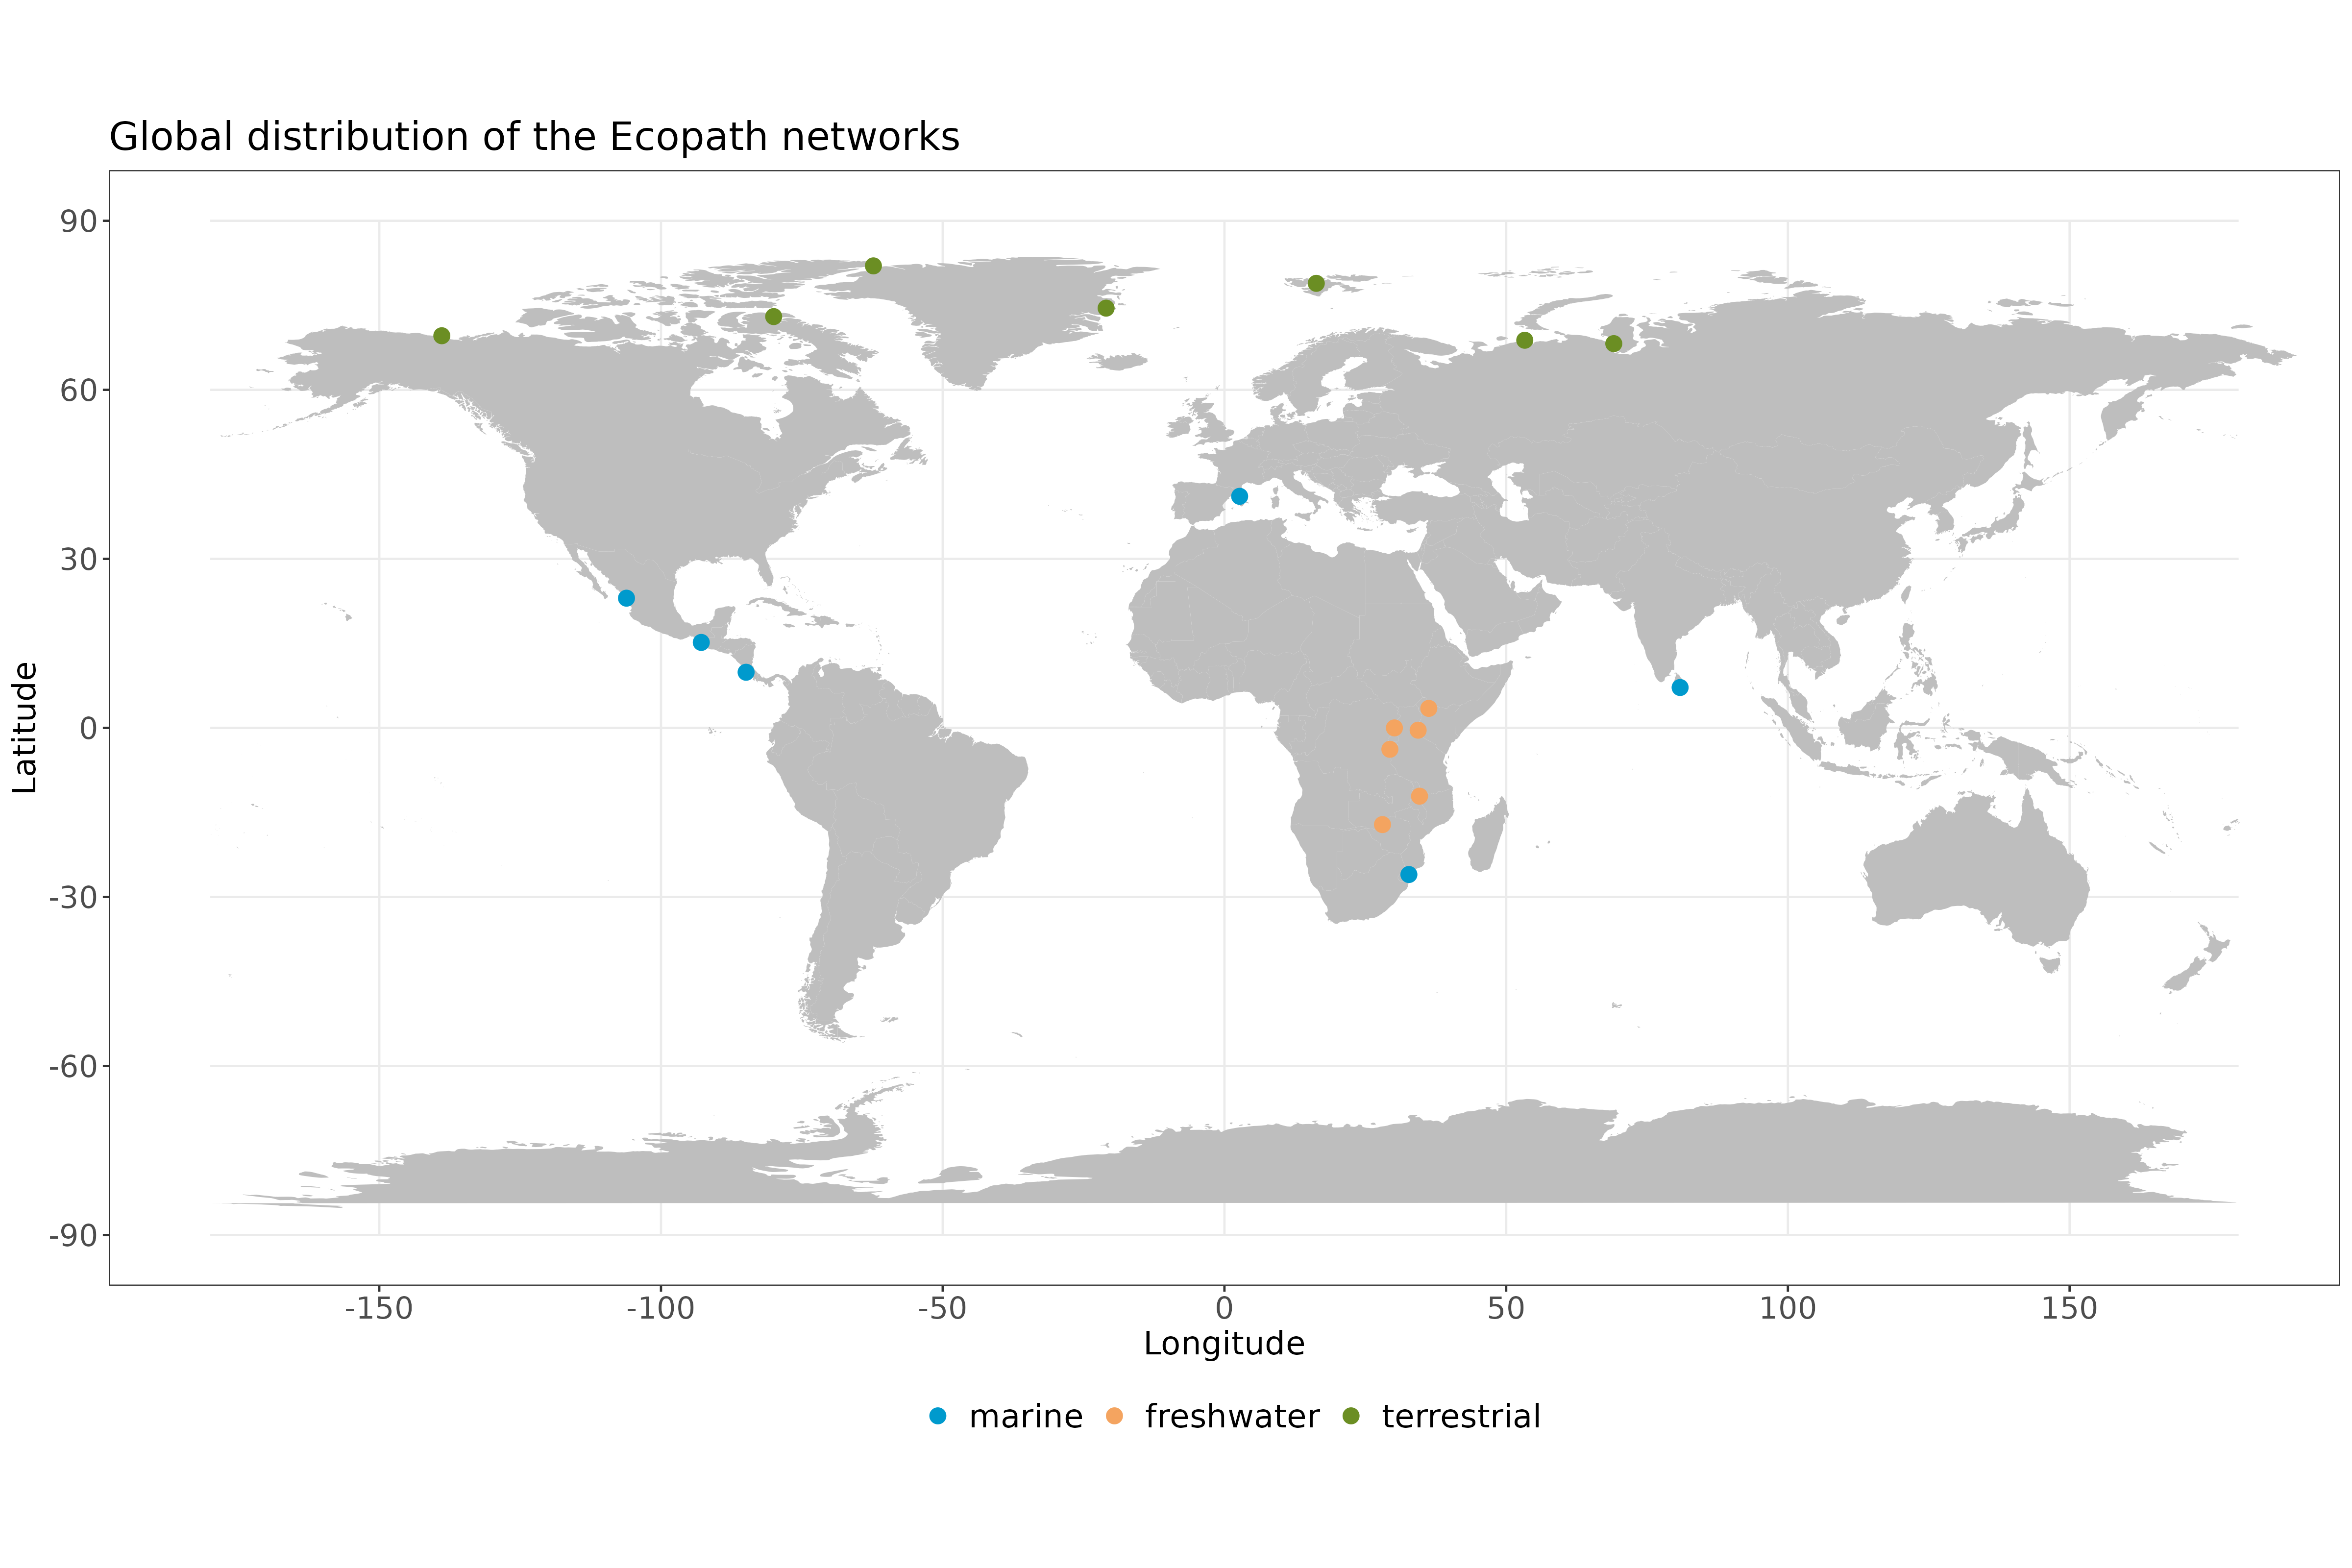
\includegraphics{figures/network_map.png}
\caption{This is the map of networks.}\label{fig:map}
}
\end{figure}

These 19 networks (fig.~\ref{fig:map}) span over different kind of
ecosystems (e.g.~marine, freshwater and terrestrial) with many different
taxas and trophic guilds (e.g.~mammal carnivores, mammal herbivores,
birds, pelagic and demersal carnivorous fish, pelagic and demersal
herbivorous fish, invertebrates, etc.). It is not uncommon for the nodes
in Ecopath networks to represent functional groups and not a specific
species. Thus, the 19 Ecopath networks were chosen based on taxonomic
resolution of the species involved. This decision was made to ensure we
could retrieve a decent estimate of organisms mean bodymass. Still, from
those 19 networks some contain functional groups but the species
involved in those nodes were well defined and pretty similar to
eachother, which made it easy to retrieve a mean bodymass for these
groups. It resulted in a list of 1380 pairwise trophic interactions
between predators and preys.

Ecopath networks come with their advantage and disadvantage. The biggest
advantage is that each network are built within the same framework
giving us a robust base to rely on.

\hypertarget{the-analysis}{%
\subsection{The analysis}\label{the-analysis}}

We first made a correspondance between the species names in the networks
with their corresponding names in their respective original article to
make sure we were working with the right species. We then proceeded to
resolve the taxonomy to work with up to date names. This allowed us to
retrieve mean body mass for each species present in our dataset. Given
the diversity of taxa present in the dataset, these species traits had
to be recovered from different databases. The mean bodymass for marine
and aquatic species were retrieve from Fishbase with length-weight
relationship, while mean bodymass for terrestrial species came from
different sources such as the GATEWAy database (Brose 2018) their
original article and grey litterature. With these mean bodymass in hand
for each species of the dataset, we computed an estimate of species
abundance (\(N\)) by dividing species biomass (\(B\)) by their mean
bodymass (\(M\)):

\[ N = \frac{B}{M} \]

The analysis were performed in a Bayesian framework with stan version
2.21.0 via the package rstan in R version 4.2.2. We proceeded to fit the
models to the data and parametrized each of the parameters per model
respectively. We then made predictions on the data with the parametrized
models and followed with a ranking using a leave-one-out method adapted
to our Bayesian framework. We also computed the bayesian R² (Gelman
\emph{et al.} 2019) for each model.

\begin{longtable}[]{@{}
  >{\centering\arraybackslash}p{(\columnwidth - 4\tabcolsep) * \real{0.3333}}
  >{\centering\arraybackslash}p{(\columnwidth - 4\tabcolsep) * \real{0.3333}}
  >{\centering\arraybackslash}p{(\columnwidth - 4\tabcolsep) * \real{0.3333}}@{}}
\toprule()
\begin{minipage}[b]{\linewidth}\centering
Model name
\end{minipage} & \begin{minipage}[b]{\linewidth}\centering
Model equation
\end{minipage} & \begin{minipage}[b]{\linewidth}\centering
Description
\end{minipage} \\
\midrule()
\endhead
Null model & \(F_{ij} = K\) & The first model acts as a null model,
where we hypothesize that the flux of biomass between a prey \(i\) and
its predator \(j\) (F\_\{ij\}) can be explained by a constant (\(K\))
which is a parameter. \\
General mass-action & \(F_{ij} = \alpha \times B_i \times N_j\) & The
second model suggests that the flux of biomass between a prey \(i\) and
its predator \(j\) can be explained by a general mass action processus
which depends on the abundance of the predator (\(N_j\)), the available
biomass of the prey (\(B_i\)) and a general space clearance rate as
parameter (\(\alpha\)). \\
Predator-specific mass-action &
\(F_{ij} = \alpha_{j} \times B_i \times N_j\) & The third model suggests
that the flux of biomass between a prey \(i\) and its predator \(j\)
still can be explained by a mass action processus which depends on the
abundance of the predator (\(N_j\)), the available biomass of the prey
(\(B_i\)) but with predator-specific space clearance rate parameters
(\(\alpha\)). \\
Saturated mass-action with handling time &
\(F_{ij} = \displaystyle\frac{\alpha_j \times B_i \times N_j}{1 + h_j \times \alpha_j \times sumB \times N_j}\)
& The fourth model hypothesize that the flux of biomass between a prey
\(i\) and its predator \(j\) is explained by a predator-specific space
clearance rate and an effect of saturation with the handling time of the
predator (\(h_j\)) both as parameter and the total amount of biomass
available of all the preys of the predator \(j\) (\(sumB\)). \\
\bottomrule()
\end{longtable}

\hypertarget{references}{%
\section*{References}\label{references}}
\addcontentsline{toc}{section}{References}

\hypertarget{refs}{}
\begin{CSLReferences}{1}{0}
\leavevmode\vadjust pre{\hypertarget{ref-Brose2018GloDat}{}}%
Brose, U. (2018). GlobAL daTabasE of traits and food Web Architecture
(GATEWAy) version 1.0.

\leavevmode\vadjust pre{\hypertarget{ref-Brown2003EcoFoo}{}}%
Brown, J.H. \& Gillooly, J.F. (2003).
\href{https://doi.org/10.1073/pnas.0630310100}{Ecological food webs:
High-quality data facilitate theoretical unification}. \emph{Proceedings
of the National Academy of Sciences}, 100, 1467--1468.

\leavevmode\vadjust pre{\hypertarget{ref-Christensen2005EcoEco}{}}%
Christensen, V., Walters, C. \& Pauly, D. (2005). Ecopath with Ecosim: A
User's Guide. \emph{Fisheries Centre, University of British Columbia,
Vancouver, Canada and ICLARM, Penang, Malaysia}, 12.

\leavevmode\vadjust pre{\hypertarget{ref-DeLong2021PreEco}{}}%
DeLong, J.P. (2021). \emph{Predator Ecology: Evolutionary Ecology of the
Functional Response}. Oxford University Press.

\leavevmode\vadjust pre{\hypertarget{ref-Gelman2019RsqBay}{}}%
Gelman, A., Goodrich, B., Gabry, J. \& Vehtari, A. (2019).
\href{https://doi.org/10.1080/00031305.2018.1549100}{R-squared for
Bayesian Regression Models}. \emph{The American Statistician}, 73,
307--309.

\leavevmode\vadjust pre{\hypertarget{ref-Hirt2017GenSca}{}}%
Hirt, M.R., Jetz, W., Rall, B.C. \& Brose, U. (2017).
\href{https://doi.org/10.1038/s41559-017-0241-4}{A general scaling law
reveals why the largest animals are not the fastest}. \emph{Nature
Ecology \& Evolution}, 1, 1116--1122.

\leavevmode\vadjust pre{\hypertarget{ref-Jordano2016ChaEco}{}}%
Jordano, P. (2016).
\href{https://doi.org/10.1371/journal.pbio.1002559}{Chasing Ecological
Interactions}. \emph{PLOS Biology}, 14, e1002559.

\end{CSLReferences}

\end{document}
